\documentclass[11pt]{article}

% ============================================================================
%  The Second Loop — arXiv preprint (draft)
%  Compile: pdflatex main && bibtex main && pdflatex main && pdflatex main
%  Every number in this paper is a verbatim output of a committed experimental
%  run; see the three companion repositories linked in the footnote on page 1.
% ============================================================================

\usepackage[margin=1in]{geometry}
\usepackage{amsmath,amssymb}
\usepackage{booktabs}
\usepackage{graphicx}
\usepackage{xcolor}
\usepackage{microtype}
\usepackage[hidelinks]{hyperref}
\usepackage{caption}
\usepackage{enumitem}
\usepackage[numbers]{natbib}   % numeric citations, but \citet/\citep available

\emergencystretch=1em          % absorb the occasional overfull line

\graphicspath{{figs/}}

\newcommand{\todo}[1]{\textcolor{red}{[\textbf{TODO:} #1]}}
\newcommand{\scar}{scar\nobreakdash-survival rate}

\title{\textbf{The Second Loop: Durable Correction of Memorized Errors in
Frozen Language Models}}

\author{
  Serghei Brinza\\
  ORCID: 0009-0006-3605-1434\\
  Independent Researcher\\
  \texttt{brinzaengineeringai@gmail.com}
}
\date{\today}

\begin{document}
\maketitle

\begingroup
\renewcommand\thefootnote{}\footnotetext{%
Code and data for all six experiments:
\href{https://github.com/SergheiBrinza/scar-survival}{scar-survival} (Part~1),
\href{https://github.com/SergheiBrinza/external-grounding}{external-grounding} (Part~2),
\href{https://github.com/SergheiBrinza/thin-channel}{thin-channel} (Part~3).
Interactive result viewers:
\href{https://huggingface.co/spaces/Laborator/second-loop}{huggingface.co/spaces/Laborator/second-loop}.}
\endgroup

\begin{abstract}
A frozen language model that has memorized a wrong fact repeats it even when the
correct fact is placed in its context. We study whether such an error can be
corrected \emph{durably} --- surviving a full process reload --- without
touching a single weight, and where the criterion of truth for such a correction
must live. We introduce the \textbf{\scar{}}: the fraction of trap facts on
which an external correction mechanism keeps beating the model's memorized
instinct across $N$ full reloads, scored by an independent semantic judge over
the generated answer. On a frozen Qwen2.5-3B-Instruct subject, a per-fact
notebook with contrastive decoding turns $0/14$ correct answers into $14/14$ and
holds them across ten reloads --- 100\% under a deliberately deterministic setup
(frozen weights, static notebook, greedy decoding) --- and under
stochastic-decoding stress (700 samples at temperature 0.7), with 92.9\% under
up to $+500$ entries of notebook ballast. The mechanism has one sharp failure mode: it
is \emph{blind to truth}. A single plausible lie placed next to the truth halves
survival to 50\%. A gatekeeper built from a same-family model cannot close the
gap --- it inherits the subject's blind spots and caps at 64.3\%, exactly its
own accuracy --- whereas a gatekeeper grounded in live Wikipedia plus targeted
retrieval engineering restores 92.9\% ($13/14$), and 100\% once one genuinely
ambiguous trap is disambiguated. The metric ports across three models and two
fact domains (100\% in all six cells, 540 answers) and discriminates a real
correction from cosmetic and placebo variants (100\% / 0\% / 14.3\%). A separate
probe asks the opposite question --- how rarely external truth can arrive before
a self-calibrating frozen forecaster drifts --- over 1{,}646 resolved
ForecastBench questions and eleven reveal schedules: any finite contact holds;
only zero contact fails. We read the whole arc through Tarski's undefinability
of truth as an organizing analogy: neither the subject nor its same-family copy
can supply a working criterion of truth; a properly integrated external source
can.
\end{abstract}

% ---------------------------------------------------------------------------
\section{Introduction}
% ---------------------------------------------------------------------------

Instruction-tuned language models carry \emph{memorized instincts}: firmly
encoded answers that the model emits with high confidence. When such an instinct
is wrong --- the tallest mountain measured base-to-peak, the first animals sent
to space, the exact wording of a famous film line --- the model repeats the error
even when the correct fact is available to it in context. The standard remedy,
weight editing or fine-tuning, changes the object we are trying to study and
raises its own durability questions.

This paper asks a narrower and, we argue, more fundamental question. Suppose the
model is a \emph{frozen subject}: its weights never change. Can we correct a
memorized error with an external mechanism, and will that correction be
\emph{durable}: specifically, will it survive a full process reload of the
model, or is it only a cosmetic effect that vanishes with process memory? We
call a durable correction a \textbf{scar}, and we call the whole research program
the \textbf{Second Loop}: correction that closes back on itself and holds across
reloads.

We make the following contributions.

\begin{enumerate}[leftmargin=1.4em,itemsep=2pt]
\item \textbf{A metric.} The \scar{} (Section~\ref{sec:metric}): the fraction of
working traps on which the mechanism keeps beating the instinct across $N$ full
reloads, scored by an independent semantic judge over the actually generated
answer.

\item \textbf{A mechanism and its failure mode} (Section~\ref{sec:exp1}, Experiment~1). A
per-fact notebook plus contrastive decoding lifts a frozen 3B model from $0/14$
to $14/14$ and holds 100\% across ten reloads, but collapses to 50\% when the
notebook is polluted with a plausible lie. The mechanism is blind to truth.

\item \textbf{Where the truth criterion must live}
(Section~\ref{sec:grounding}, Experiments~2--3). A gatekeeper made from a same-family model caps at
64.3\%: it shares the subject's blind spots. Replacing it with a real external
source (live Wikipedia) plus targeted retrieval engineering restores 92.9\%, and
100\% after disambiguating one trap. We connect this to Tarski's undefinability
of truth.

\item \textbf{Metric validation} (Section~\ref{sec:validation}, Experiments~4--5). The metric
ports across three models and two fact domains (100\% in all six cells) and
discriminates a real scar from cosmetic and placebo controls (100\% / 0\% /
14.3\%).

\item \textbf{The opposite bound} (Section~\ref{sec:thin}, Experiment~6). Using resolved
forecasting questions as a stream of ``truth from the future,'' we sweep how
rarely external feedback can arrive before a self-calibrating frozen system
drifts. The collapse is binary: any finite contact holds; only zero contact
fails.
\end{enumerate}

A note on honesty of claims, stated up front because it governs how every number
below should be read. Several headline figures are 100\%. Under a frozen model,
a static notebook on disk, and greedy decoding, a full process reload
deterministically reproduces the same state, so 100\% survival across reloads is
partly a property of that determinism. The contribution lies elsewhere:
(i) that the protocol is portable across models and domains
(Section~\ref{sec:validation}), (ii) that it discriminates real from fake
interventions (Section~\ref{sec:validation}), and (iii) that it exposes and then
closes a real failure mode --- memory pollution --- with an external source of
truth (Section~\ref{sec:grounding}).

% ---------------------------------------------------------------------------
\section{Related Work}
% ---------------------------------------------------------------------------

\paragraph{Knowledge editing.} Methods such as ROME~\cite{rome} and
MEMIT~\cite{memit} edit facts by modifying weights.
Our setting is deliberately complementary: the weights are frozen and the
correction lives entirely outside the model, which lets us ask the durability
question without confounding it with weight-update stability.
Beyond single-edit stability, sequential editing degrades the edited model
\citep{gupta2024editing} and edits ripple unpredictably into related facts
\citep{cohen2024ripple}, an added motivation for keeping corrections outside
the weights entirely.

\paragraph{Knowledge conflicts and context faithfulness.}
When an in-context fact contradicts a model's parametric memory, models
frequently revert to the memorized answer. This context--memory conflict is
documented from entity-substitution studies \citep{longpre2021entity} through
controlled behavioral analyses \citep{xie2024adaptive}, and is systematized in
the survey of \citet{xu2024knowledge}. Our traps are a deliberately adversarial
instance: fourteen facts on which the subject's parametric prior confidently
beats a correct in-context fact. The failure mode of \S4 (the corrector
amplifying a plausible distractor) is the inter-context variant of the same
conflict, arising when the notebook itself carries contradictory entries.

\paragraph{Contrastive and context-faithful decoding.}
Contrastive decoding was introduced as a generation-quality objective
\citep{li2023contrastive} and later directed at factuality, either by
contrasting layers \citep{chuang2024dola} or, closest to us, by
contrasting a run with and without the context, as in context-aware decoding
\citep{shi2024trusting}; CK-PLUG~\cite{ckplug} and DeCK~\cite{deck} refine this
contrast for knowledge editing. Our mechanism is a direct implementation of this
family; our contribution is the durability protocol around the decoder:
reload survival, stress loads, and discrimination controls. Our
Confidence Gain indicator (Section~\ref{sec:exp1}) follows the
knowledge-consistency signal of CK-PLUG~\cite{ckplug}.

\paragraph{Memory corruption in retrieval-augmented systems.}
Our counterfeit-notebook stress test is a manual instance of corpus poisoning:
a handful of injected passages reliably steers retrieval-augmented answers
\citep{zhong2023poisoning, zou2024poisonedrag}, and certified defenses respond
by aggregating over isolated passages \citep{xiang2024certifiably}. Two
differences in aim: our injected lie is not optimized (a single plausible
decoy suffices to halve survival), and our defense is scored end-to-end by
scar survival across reloads rather than by retrieval metrics. The identity of
\S5 --- the defense ceiling equals the verifier's accuracy --- holds exactly
in our setting; with $n=14$ we read this as a hypothesis about the mechanism,
not a law.
Broader treatments of these risks place corpus poisoning within a wider
trustworthiness agenda for retrieval-augmented systems
\citep{ni2025trustworthy}.
Closest in spirit to our gatekeeper, \citet{si2025secon} pair semantic filtering
of the corpus with a conflict-aware stage that screens query, candidate answer
and retrieved evidence for contradiction before generation, a design that
independently arrives at the same decomposition as our conflict detector plus
arbiter, though scored by generation robustness rather than by survival across
reloads.

\paragraph{Limits of self-correction.}
Intrinsic self-correction --- a model revising its own output without new
information --- largely fails on reasoning tasks \citep{huang2024cannot}, and
surveys locate reliable correction in external feedback
\citep{pan2024automatically, kamoi2024when}. Our clone-arbiter result is the
fact-level, mechanistic version of that conclusion: a same-family verifier
inherits the subject's blind spots and caps exactly at its own accuracy
(\S5), while an external source restores nearly full survival.

\paragraph{Retrieval-augmented grounding.} Part~2 grounds a gatekeeper in live
Wikipedia retrieval~\cite{rag}.
Our finding there is specifically about the \emph{precision/recall operating
point} of the retriever as the binding constraint, not retrieval in general.

\paragraph{Calibration and forecasting.} Part~3 uses ForecastBench~\cite{forecastbench}
as a stream of resolved binary questions and applies per-topic Beta calibration.

% ---------------------------------------------------------------------------
\section{The Scar-Survival Rate}
\label{sec:metric}
% ---------------------------------------------------------------------------

Let $T$ be a set of \emph{working traps}: questions on which the frozen model
$M$, run in its clean regime (no correction mechanism), confidently produces the
wrong answer. Let $\mathrm{Mem}$ be an external memory of correct facts, each
tagged as ``truth that overrides the memorized answer''; let $\mathrm{Mech}$ be a
correction mechanism running on top of $M$ (contrastive decoding, retrieval
augmentation, $\dots$); let $N$ be the number of full process reloads; and let
$J$ be an independent semantic judge that labels each answer \texttt{correct} or
\texttt{incorrect} against the reference fact. For each trap $t$ and reload $n$,
$\text{answer}(t,n)=M(\mathrm{Mech},\mathrm{Mem})(t)$ and
$\text{verdict}(t,n)=J(\text{answer}(t,n),\text{gold}(t))$. Then
%
\begin{equation}
\text{scar-survival rate} \;=\;
\frac{\bigl|\{\, t\in T : \forall\, n\in\{1,\dots,N\},\ \text{verdict}(t,n)=\texttt{correct} \,\}\bigr|}{|T|}.
\end{equation}
%
Two design choices matter. First, each reload $n$ is a \emph{separate operating
system process}: the model is fully unloaded and reloaded from scratch and the
notebook is re-read from disk, so a ``cosmetic'' correction that lives only in
process memory cannot survive. Second, scoring is done by a semantic judge over
the actual generated answer, not by keyword matching or by a token-level
probability metric; Section~\ref{sec:exp1} shows why the latter is unreliable.
Throughout this paper $N=10$ and $J$ is Qwen2.5-7B-Instruct.

% ---------------------------------------------------------------------------
\section{Experiment 1: The Scar Mechanism}
\label{sec:exp1}
% ---------------------------------------------------------------------------

\paragraph{Setup.} The frozen subject is Qwen2.5-3B-Instruct, run on a single
RTX~3090~Ti. We screened both Qwen2.5-7B-Instruct and Qwen2.5-3B-Instruct over the
same 58 candidate traps (myths, geography, quotations, niche facts, ``false
friends'') with the same automatic marker-based classifier, which labels each
answer \texttt{correct}, \texttt{wrong\_instinct}, or \texttt{ambiguous}. Under
that single criterion the two models fire the memorized error at the same rate
--- $6/58 = 10.3\%$ each --- but they differ in how cleanly they get the rest
right: the 7B leaves no ambiguous answers, whereas the 3B leaves 7, so 13/58
($22.4\%$) of its answers are not unambiguously correct. We chose the 3B because
it also hallucinates its own wrong answer readily, which is what the mechanism
must override. A manual review of all 58 of the 3B's answers (not applied to
the 7B) yields the \textbf{14 working traps} used throughout this paper.
Thirteen come from the fired and ambiguous buckets; one (\#46) was promoted from
an answer the classifier scored \texttt{correct} because the generated text
contradicts itself arithmetically: it answers ``No,'' then reports a Venusian day
of 243 Earth days against a Venusian year of approximately 225, yet calls the day
\emph{shorter} than the year. The external memory is a
notebook holding, for each trap, the correct fact.

\paragraph{Correction mechanism.} At each decoding step the model is evaluated
twice --- with the fact in context and without it (pure instinct) --- and the
next-token distribution is shifted toward the fact:
\begin{equation}
\text{logits} \;=\; (1+\alpha)\cdot \text{logits}_{\text{with fact}} \;-\; \alpha\cdot \text{logits}_{\text{instinct}},
\qquad \alpha = 1.0,
\end{equation}
with a plausibility threshold $\beta=0.1$ that prevents amplifying low-probability
nonsense. We also report \textbf{Confidence Gain} (after CK-PLUG~\cite{ckplug}), the
increase in probability mass on the correct answer,
$P_{\text{contrastive}}-P_{\text{instinct}}$, as an indicator of override
strength.

\paragraph{Three modes.} Scored by the independent 7B judge over 14 traps:
pure instinct gives $0/14$ (0\%); the plain notebook (fact in context) gives
$14/14$ (100\%); contrastive decoding also gives $14/14$ (100\%), with a mean
Confidence Gain of $+0.744$. The distinction between the two 100\% columns is
qualitative: on trap~\#37 (``first animal in space'') the fact-in-context barely
moved the choice ($P=0.017$), whereas contrastive raised it to $0.899$: the
difference between reading off a crib and a genuine intervention.

\paragraph{Scar survival across ten reloads.} Running the strict protocol (each
cycle a separate process), the \scar{} is 100\% in every one of the ten cycles
($14/14$ each time), and the Confidence Gain is bit-for-bit $0.7439$ in every
cycle (Figure~\ref{fig:scar}). As stated in the introduction, this exactness is
a consequence of the deterministic setup; the value of the run is that it
establishes the protocol and the baseline against which the stress tests and the
discrimination controls (Section~\ref{sec:validation}) are read.

\begin{figure}[t]
\centering
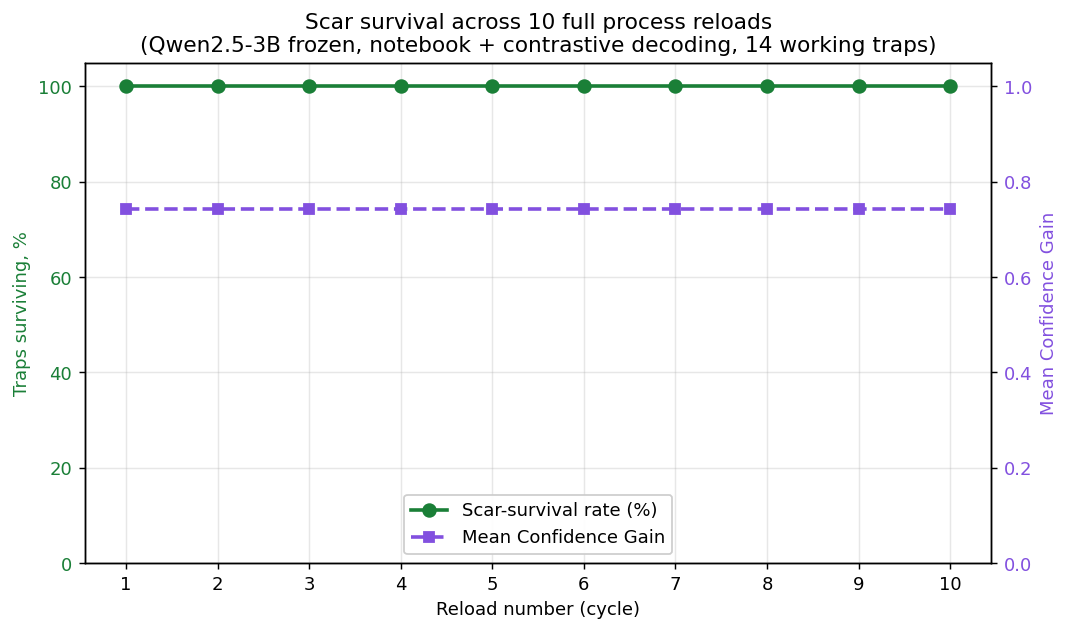
\includegraphics[width=0.62\linewidth]{fig1_scar_survival.png}
\caption{Scar survival across ten full process reloads (Experiment 1):
$14/14$ traps held in every cycle.}
\label{fig:scar}
\end{figure}

\paragraph{Stress tests.} We then probe the override under pressure on the
notebook itself (Table~\ref{tab:stress}, Figure~\ref{fig:stress}). It survives a
growing notebook (up to $+500$ ballast entries, 92.9\%) and stochastic decoding
(temperature $0.7$, $700$ samples, 100\%), and it survives even the stickiest
instincts (12 traps with $P_{\text{instinct}}\approx 0$, 100\%). It fails under a
\emph{noisy notebook}: with two to three plausible distractor entries next to the
truth, survival drops to $50\%$ ($7/14$). Under this load the model copied the
false distractor verbatim (``3 seconds,'' ``K2,'' ``Play it again, Sam,''
``Laika,'' ``Steamboat Willie''), and on two traps the Confidence Gain went
negative.

\begin{table}[t]
\centering
\caption{Experiment 1 stress tests (survival by 7B judge over the generated
answer).}
\label{tab:stress}
\begin{tabular}{lcc}
\toprule
Load & Survival & Verdict \\
\midrule
Baseline (clean, 10 reloads)                 & 100\%        & --- \\
1. Growing notebook ($+50/100/200/500$)      & 92.9\%       & holds; Gain stable $0.65$--$0.72$ \\
2. Noisy memory (2--3 distractors)           & 50\% ($7/14$)& \textbf{fails} \\
3. Stochasticity ($\text{temp}{=}0.7$, 700 samples) & 100\% & holds, no spread \\
4. Sticky instincts ($P_{\text{instinct}}\approx 0$, 12 traps) & 100\% & holds, Gain $+0.58$ \\
\bottomrule
\end{tabular}
\end{table}

\begin{figure}[t]
\centering
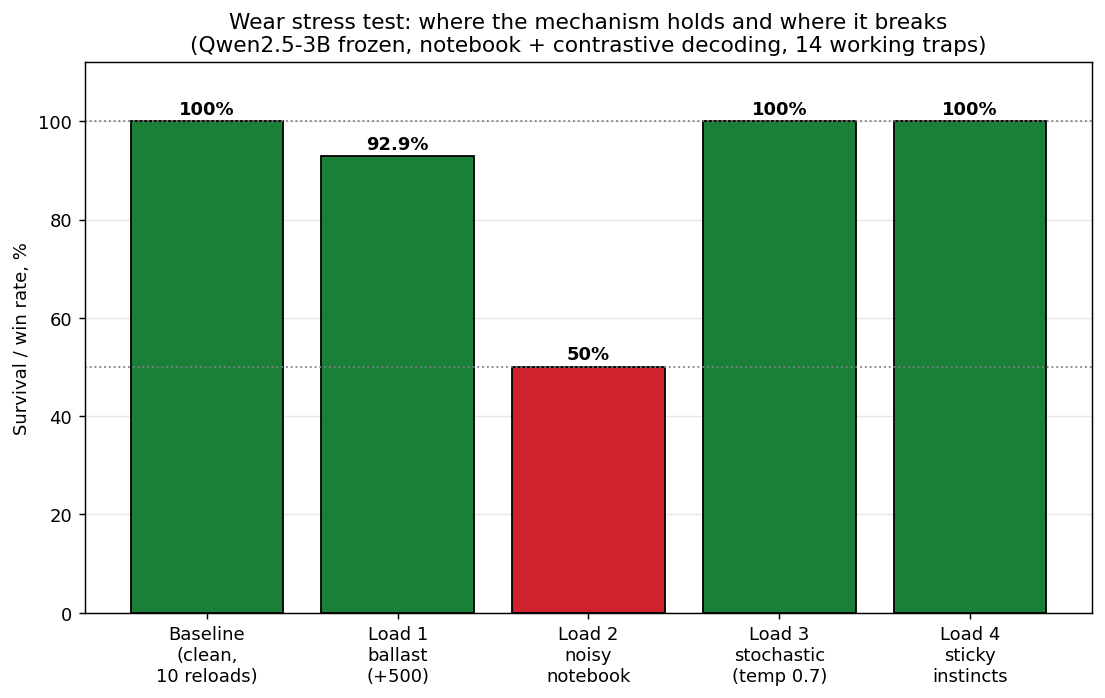
\includegraphics[width=0.85\linewidth]{fig2_stress.png}
\caption{Where the mechanism holds and where it breaks (Experiment 1). Memory
pollution, not wear, is the failure mode.}
\label{fig:stress}
\end{figure}

\paragraph{A methodological caveat.} Confidence Gain overestimates robustness
under noise. It compares the correct answer against a single canonical wrong one,
but free generation can latch onto a \emph{third} distractor outside that
comparison (on trap~\#20 the metric read $+0.90$ while the model generated
``K2''). The honest measure is therefore the semantic judge over the actual
answer; we keep Confidence Gain only as an indicator of override strength, not as
proof of correctness. This is why the metric in Section~\ref{sec:metric} is
defined over $J$, not over probabilities.

\paragraph{Takeaway.} The ceiling of the mechanism is \emph{notebook quality},
not its size, decoding randomness, or instinct strength. Contrastive decoding
breaks through the most stubborn instinct, but it will amplify a plausible lie
sitting next to the truth just as readily, especially when the lie coincides
with the model's own instinct. This motivates Part~2.

% ---------------------------------------------------------------------------
\section{Guarding the Notebook: Where the Truth Criterion Must Live}
\label{sec:grounding}
% ---------------------------------------------------------------------------

The failure mode of Section~\ref{sec:exp1} is memory pollution. We place a
\emph{gatekeeper} at the entrance to the notebook whose job is to reject false or
conflicting entries before they reach the corrector. The gatekeeper has three
parts: a conflict detector (pairwise comparison of entries for the same
question), an arbiter (which adjudicates flagged conflicts), and a quarantine
(rejected entries are isolated from the working notebook). The conflict detector
caught the contradiction in every noisy entry ($14/14$); the interesting variable
is the \emph{arbiter}.

\paragraph{Guardian 1.0 --- a same-family arbiter (Experiment 2).} When the
arbiter is a second model of the same family (Qwen2.5-7B judging entries for a
Qwen2.5-3B subject), survival rises from the polluted 50\% only to 64.3\% ($9/14$).
Crucially, the protected-case survival (64.3\%) exactly equals the fraction of
traps on which the arbiter itself kept the correct fact (64.3\%): the defense
ceiling equals the accuracy of the verifier (Figure~\ref{fig:guard1}). The arbiter failed on precisely the
stickiest facts where the subject failed (Mauna~Kea; the length of a day on
Venus; fruit flies vs.\ Laika; the misquotes from \emph{Snow White} and
\emph{Casablanca}), because a same-family model shares the subject's blind spots.
On one trap (\#46) the defense even regressed, quarantining a correct fact it
judged false. A clone cannot supply the truth criterion.

\begin{figure}[t]
\centering
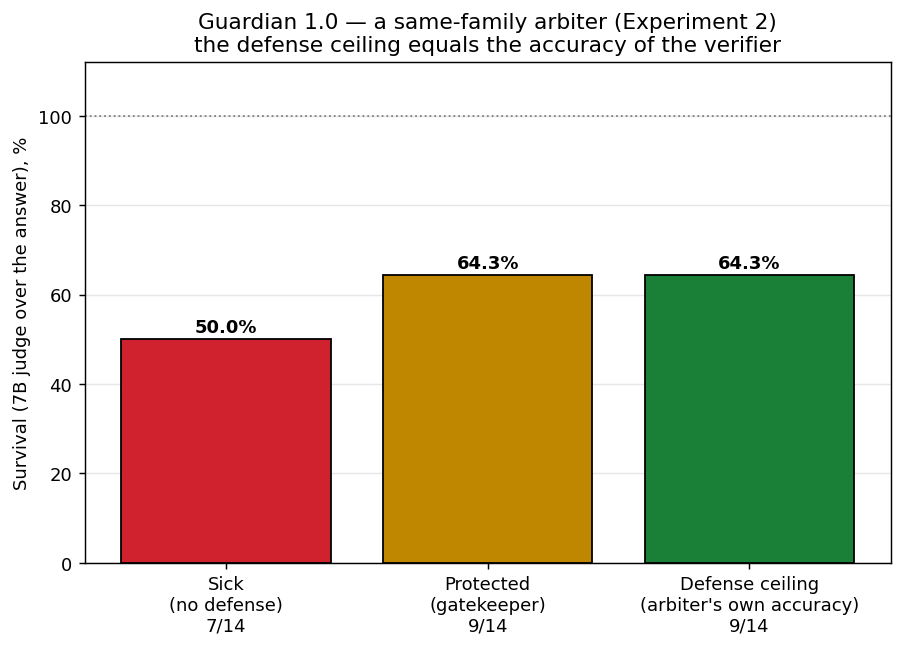
\includegraphics[width=0.55\linewidth]{fig3_guardian_v1.png}
\caption{The clone ceiling: survival under Guardian 1.0 (64.3\%) exactly equals
the fraction of traps on which the arbiter itself kept the correct fact ($9/14$).
The defense ceiling equals the accuracy of the verifier.}
\label{fig:guard1}
\end{figure}

\paragraph{Guardian 2.0 --- an external source (Experiment 3).} We replace the
model arbiter with live Wikipedia retrieval and a grounded reader. The survival
arc is shown in Table~\ref{tab:arc} and Figure~\ref{fig:arc}. A raw external
source lifts the ceiling from 64.3\% to 71.4\% by curing exactly the clone's blind
spots. A blunt ``make retrieval stronger'' pass does nothing (71.4\%$\to$71.4\%): it
merely trades false admissions for false quarantines: a precision/recall wall.
The gain comes instead from three \emph{targeted} fixes: (i) a verbatim-match
check for quote facts; (ii) a relevance gate that rejects coincidental namesake
articles (a query about a \emph{Snow White} line is no longer ``confirmed'' by
the 2012 film \emph{Mirror Mirror}); and (iii) a soft threshold that keeps a
doubtful truth at reduced trust instead of quarantining it, reserving quarantine
for entries the source explicitly contradicts. These reach 85.7\%. A final
calibration of the relevance gate, plus rewriting one genuinely ambiguous trap,
reaches 100\%.

\begin{table}[t]
\centering
\caption{Full survival arc under a polluted notebook (Experiments 1--3), scored
by the independent judge over the generated answer.}
\label{tab:arc}
\begin{tabular}{llc}
\toprule
Version & Verifier & Scar survival \\
\midrule
Sick (no defense)      & ---                       & 50.0\% \\
Guardian 1.0           & model arbiter (clone)     & 64.3\% \\
Guardian 2.0           & Wikipedia (retrieval)     & 71.4\% \\
Guardian 2.1           & wiki + brute strengthening & 71.4\% \\
Guardian 2.2           & wiki + three targeted fixes & 85.7\% \\
\textbf{Guardian 2.3}  & wiki + final calibration  & \textbf{100.0\%}$^\dagger$ \\
\bottomrule
\end{tabular}

{\footnotesize $\dagger$ includes disambiguating one trap (\#46); without it,
92.9\% (13/14).}
\end{table}

\begin{figure}[t]
\centering
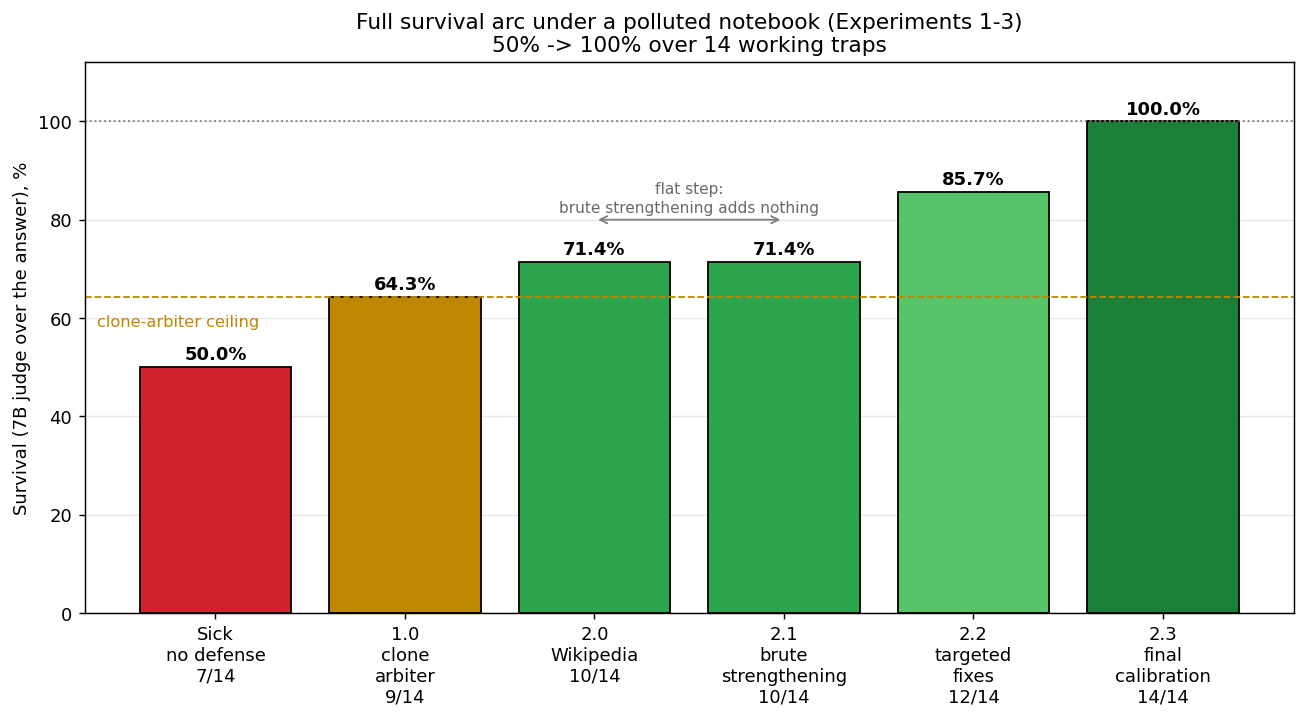
\includegraphics[width=0.7\linewidth]{fig4_guardian_v2_arc.png}
\caption{From 50\% to 92.9\%, and to 100\% after disambiguating one trap:
healing a polluted notebook with a real external source of truth plus targeted
retrieval engineering (Experiment 3).}
\label{fig:arc}
\end{figure}

\paragraph{Interpretation.} Three lessons. (a) The truth-blindness limit is
closed by a \emph{combination} --- external source \emph{and} retrieval
engineering \emph{and} clean, unambiguous traps --- not by any single trick;
remove one and the ceiling drops. (b) Not every trade-off is fundamental: the
apparent precision/recall conflict at 2.1 dissolved once the tool was made
smarter (keep by default, drop only explicit namesakes). (c) A real external
source audits the \emph{test set}, not just the model: trap~\#46 (``is a day on
Venus longer than its year?'') was ambiguous between the sidereal day (243~days,
longer than the 225-day year) and the solar day ($\sim$117~days, shorter); the
clone never noticed, but the external channel ``confirmed'' both readings because
both are true, forcing us to disambiguate the question.
We read this through Tarski's undefinability of truth \cite{tarski1936} as an
organizing analogy, not a formal claim: a sufficiently expressive system cannot
define its own truth predicate, and in our setting neither the subject nor its
same-family copy could supply a working criterion of truth; an external
source, properly integrated, could.

% ---------------------------------------------------------------------------
\section{Does the Metric Mean Anything? Universality and Discrimination}
\label{sec:validation}
% ---------------------------------------------------------------------------

A metric that reads 100\% is only useful if it also (a) ports beyond one model
and one fact set and (b) returns \emph{low} scores on interventions that are not
real. We test both.

\paragraph{Universality (Experiment 4).} We run the full protocol on a
$3\times2$ grid: three instruction-tuned models (Qwen2.5-3B-Instruct,
Qwen2.5-7B-Instruct, Phi-3.5-mini-instruct) $\times$ two fact sets (set~A:
58~misconceptions; set~B: 20 geography/records), with 10 reloads per cell and
7--10 working traps per cell (540 answers total). The \scar{} is 100\% in every
one of the six cells. On a single RTX~3090~Ti the end-to-end run takes
$\sim$3--4~hours, dominated by repeated model loads.

\paragraph{Discrimination (Experiment 5).} On Qwen2.5-3B-Instruct we run three
regimes head-to-head, 10 reloads each (30 cycles, 420 judged answers;
Figure~\ref{fig:disc}):
\begin{itemize}[leftmargin=1.4em,itemsep=1pt]
\item \textbf{R1 --- real scar}: notebook reconnected every cycle, contrastive
decoding with the refuting fact. Result: \textbf{100\%}.
\item \textbf{R2 --- cosmetic}: cycle~1 uses the notebook, cycles 2--10 run bare
instinct. Result: \textbf{collapses to 0\%} immediately after cycle~1.
\item \textbf{R3 --- placebo}: notebook reconnected every cycle but every entry
is an irrelevant administrative sentence; contrastive idles. Result:
\textbf{14.3\%}, i.e.\ baseline chance that a trap is already answered right.
\end{itemize}
The metric returns high scores only on the real mechanism and low scores on the
two fakes, so it tracks the mechanism rather than the model's general competence.

\begin{figure}[t]
\centering
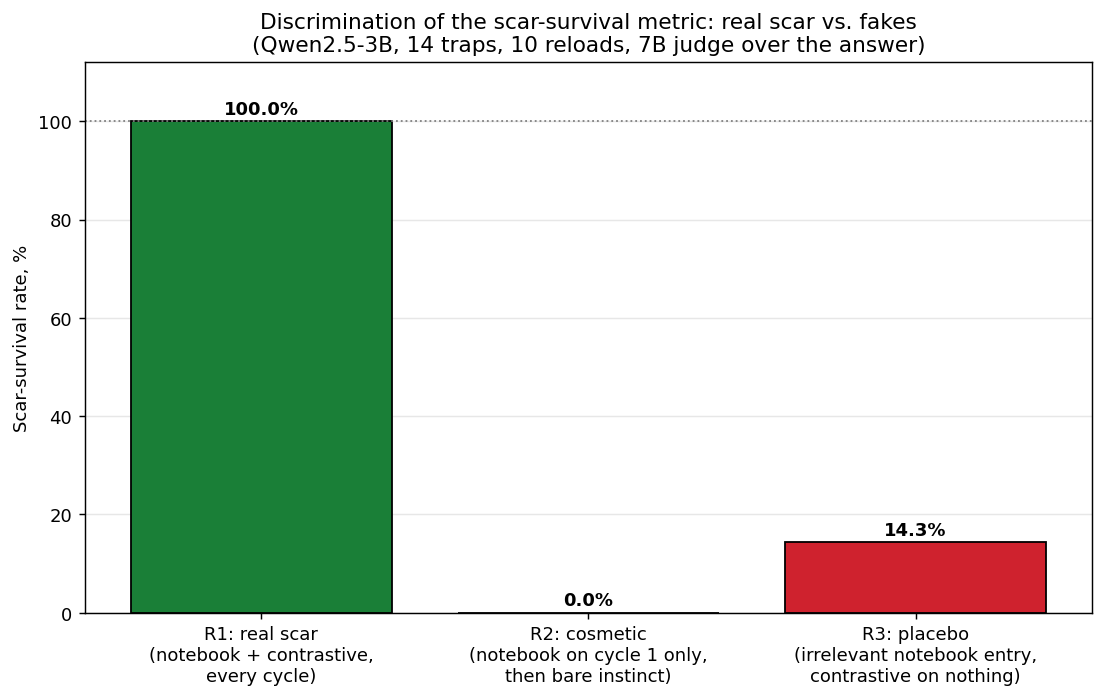
\includegraphics[width=0.6\linewidth]{fig5_discrimination.png}
\caption{Metric discrimination (Experiment 5): real scar (100\%) vs.\ cosmetic
(0\%) vs.\ placebo (14.3\%) over ten reloads.}
\label{fig:disc}
\end{figure}

% ---------------------------------------------------------------------------
\section{The Thin Channel: How Rarely Truth Can Arrive}
\label{sec:thin}
% ---------------------------------------------------------------------------

Parts 1--2 established that a live external source heals a corrupted memory.
Part~3 is a methodologically separate probe of the same wall from the opposite
side: instead of asking whether external truth can fix a frozen system, it asks
how rarely that truth can arrive before the system drifts. The setup, metric,
and object differ deliberately; what carries over is the question of where the
criterion of truth must live.

\paragraph{Setup.} We use ForecastBench --- 1{,}646 resolved binary forecasting
questions (July~2024--December~2025) --- as a stream of ``truth from the future.''
A frozen Qwen2.5-3B-Instruct emits a raw $P(\text{YES})$ for each question at its
freeze date; the outcome is hidden and revealed only on a schedule. On top of the
frozen model sits a per-topic Beta calibration (9 topics, saturation $K=10$) with
no weight updates. We split 1{,}316 train / 330 hold-out by freeze date and
report hold-out Brier score. The same stream is run independently through eleven
reveal schedules from daily to ``never.''

\paragraph{The raw model is a poor forecaster --- calibration does the work.}
On 250 questions the raw 3B has Brier $0.354$, worse than an ``always~NO''
baseline ($0.340$) and much worse than ``always topic base rate'' ($0.224$). On
the 330-question hold-out, the ablations are: raw model $0.298$; topic base-rate
only $0.189$; the Beta mixture $0.1889$. The mixture beats the raw model by
$0.109$ Brier but beats base-rate-only by only $0.0001$: essentially all of the
usable signal is the topic base rate, and the raw model contributes almost
nothing. We state this plainly, without dressing the calibrator up as a
competent forecaster.

\paragraph{The collapse is binary.} Sweeping the reveal schedule
(Table~\ref{tab:sweep}, Figure~\ref{fig:thin}), all ten \emph{finite} schedules,
from daily down to once a year, land in hold-out Brier $[0.205,0.220]$.
Only ``never'' collapses to $0.298$, bit-for-bit the raw 3B baseline. Neither
frequency nor delivered volume is the binding constraint in this regime. The
270-day schedule delivers 220 resolutions and reaches Brier $0.216$; the daily
schedule delivers 1{,}316 and reaches $0.205$. A six-fold difference in
delivered signal moves the score by $0.011$, while the gap between any finite
schedule and no contact at all is $0.08$ to $0.09$. With 9 topics at $K=10$ the
calibration saturates after a few hundred resolutions, so the experiment
separates contact from no contact and says nothing finer.

\begin{table}[!htbp]
\centering
\caption{Hold-out Brier ($N=330$) across eleven reveal schedules (Experiment 6).
Any finite contact holds; only ``never'' collapses to the raw baseline.}
\label{tab:sweep}
\begin{tabular}{lccc}
\toprule
Schedule & Period (days) & Hold-out Brier & Total revealed \\
\midrule
day       & 1   & 0.205 & 1316 \\
3 days    & 3   & 0.205 & 1315 \\
week      & 7   & 0.211 & 1313 \\
2 weeks   & 14  & 0.210 & 1313 \\
month     & 30  & 0.210 & 1277 \\
2 months  & 60  & 0.220 & 1173 \\
quarter   & 90  & 0.220 & 1022 \\
half year & 180 & 0.209 & 417 \\
270 days  & 270 & 0.216 & 220 \\
year      & 365 & 0.220 & 417 \\
\textbf{never} & --- & \textbf{0.298} & 0 \\
\bottomrule
\end{tabular}

\parbox{0.92\linewidth}{\footnotesize Total revealed is not monotone in the
period. Reveals fire on days that are multiples of the period within a fixed
535-day window, so the last effective reveal falls on day 360 for the 180-day
schedule, day 270 for the 270-day schedule, and day 365 for the 365-day
schedule; resolutions still pending when the window closes are never delivered.
Because no question resolves between days 361 and 365, the 180-day and 365-day
schedules deliver the same 417 resolutions, while the 270-day schedule delivers
only 220. The column reports how much signal reached the calibrator inside the
simulated window, not how often the schedule fires.}
\end{table}

\begin{figure}[t]
\centering
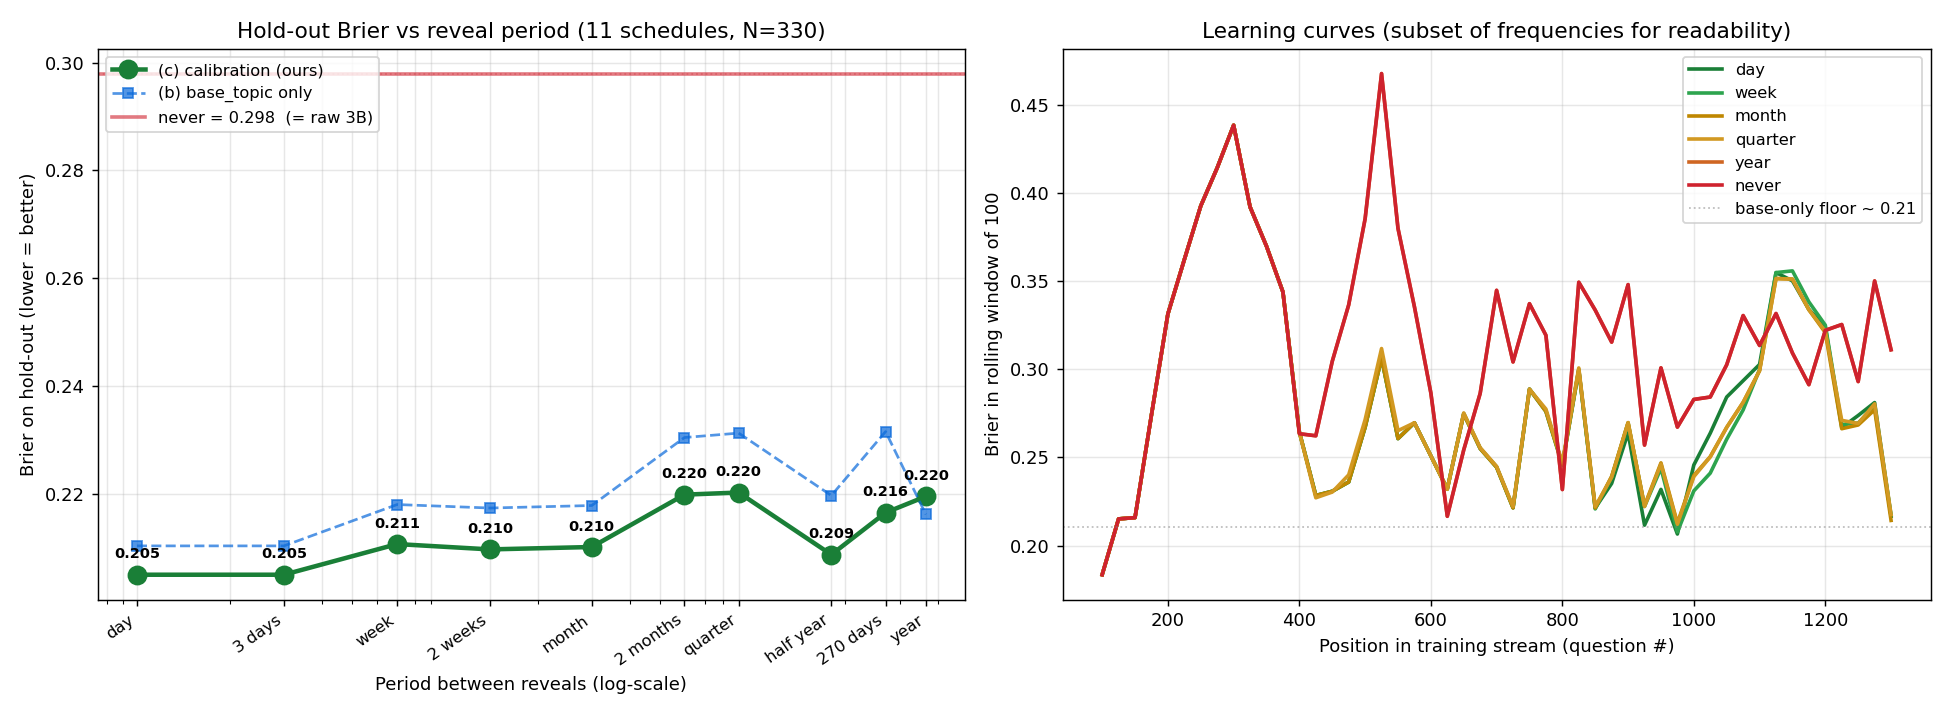
\includegraphics[width=0.9\linewidth]{fig6_thin_channel.png}
\caption{The thin channel (Experiment 6): hold-out Brier vs.\ reveal period.
Every finite schedule holds near $0.21$; only zero contact collapses to the raw
baseline $0.298$.}
\label{fig:thin}
\end{figure}

% ---------------------------------------------------------------------------
\section{Limitations and Scope of Claims}
% ---------------------------------------------------------------------------

\begin{itemize}[leftmargin=1.4em,itemsep=2pt]
\item \textbf{Determinism inflates the headline numbers.} The 100\% survival in
Experiments 1 and 4 is partly a consequence of frozen weights, a static notebook,
and greedy decoding: a process reload reproduces an identical state. The claims we
stand behind are the \emph{portability} (Experiment 4), the \emph{discrimination}
(Experiment 5), and the \emph{failure-and-repair} arc (Experiments 1--3), not the
100\% as such.
\item \textbf{Confidence Gain is not proof of correctness}; it overestimates
robustness under noise (Section~\ref{sec:exp1}). All survival numbers are scored
by a semantic judge over the generated answer.
\item \textbf{Scale.} Experiments center on a 3B subject with 14 working traps;
Experiment 4 extends to 7B and Phi-3.5-mini and to a second fact set, but the
regime is small-model, small-trap-set by design (the effect is only visible where
the model actually errs).
\item \textbf{Judge dependence.} The judge is Qwen2.5-7B-Instruct. For the
knowledge-editing traps this is adequate, but the judge is itself a model; a
human-audited subset would strengthen the claim.
\item \textbf{Thin channel is a single calibrator.} The binary-cliff result holds
for per-topic Beta calibration with 9 topics at $K=10$; a richer calibrator with
more capacity might show a graded, rather than binary, dependence on frequency.
\item \textbf{Statistical resolution.} With 14 traps every percentage moves in
steps of 7.1\%; a $14/14$ result carries an exact 95\% Clopper--Pearson lower
bound of roughly 77\%. All headline percentages should be read at that
resolution.
\end{itemize}

% ---------------------------------------------------------------------------
\section{Conclusion}
% ---------------------------------------------------------------------------

A memorized error in a frozen language model can be corrected durably, without
touching a weight, by an external notebook and contrastive decoding, but the
mechanism is blind to truth, and a single plausible lie next to the truth halves
its survival. Neither the model nor a same-family copy can supply the missing
truth criterion; a real external source can, provided its retrieval operating
point is engineered rather than merely ``strengthened.'' The \scar{} metric ports
across models and domains and discriminates real corrections from cosmetic and
placebo ones. And when external truth is the healing agent, the low-capacity
calibrator used here saturates after a few hundred resolutions: within that
regime neither arrival rate nor delivered volume separates the schedules, and
only zero contact fails. Across all three parts the same
wall recurs (a system cannot certify its own truth from inside), and the same
key opens it: a criterion supplied from outside.

% ---------------------------------------------------------------------------
\section*{Reproducibility}
% ---------------------------------------------------------------------------
Every figure and every number above is a verbatim output of a committed run.
Part~1 (Experiments 1, 4, 5): \url{https://github.com/SergheiBrinza/scar-survival}.
Part~2 (Experiments 2, 3): \url{https://github.com/SergheiBrinza/external-grounding}.
Part~3 (Experiment 6): \url{https://github.com/SergheiBrinza/thin-channel}.
Subject model Qwen2.5-3B-Instruct (frozen); independent judge Qwen2.5-7B-Instruct.
ForecastBench data is not redistributed here; see DATA.md in the thin-channel
repository for the download procedure. ForecastBench is
CC~BY-SA~4.0~\cite{forecastbench}.

\bibliographystyle{plainnat}
\bibliography{references}

\end{document}
